

\section{Integrationstest} \label{Integrationstest}
Der er lavet tre forskellige test af det samlede system, til at teste de essentielle funktioner af converteren. Det drejer sig om constant-load, gain-fase måling og load-step. For nærmere beskrivelse af hver enkelt test, henvises til dokumentationen afsnit 5.9.

På figur~\ref{fig:sche2iteration} ses et schematic for det samlede implementerede kredsløb for 2. iteration.
\begin{figure}[H]
	\center
	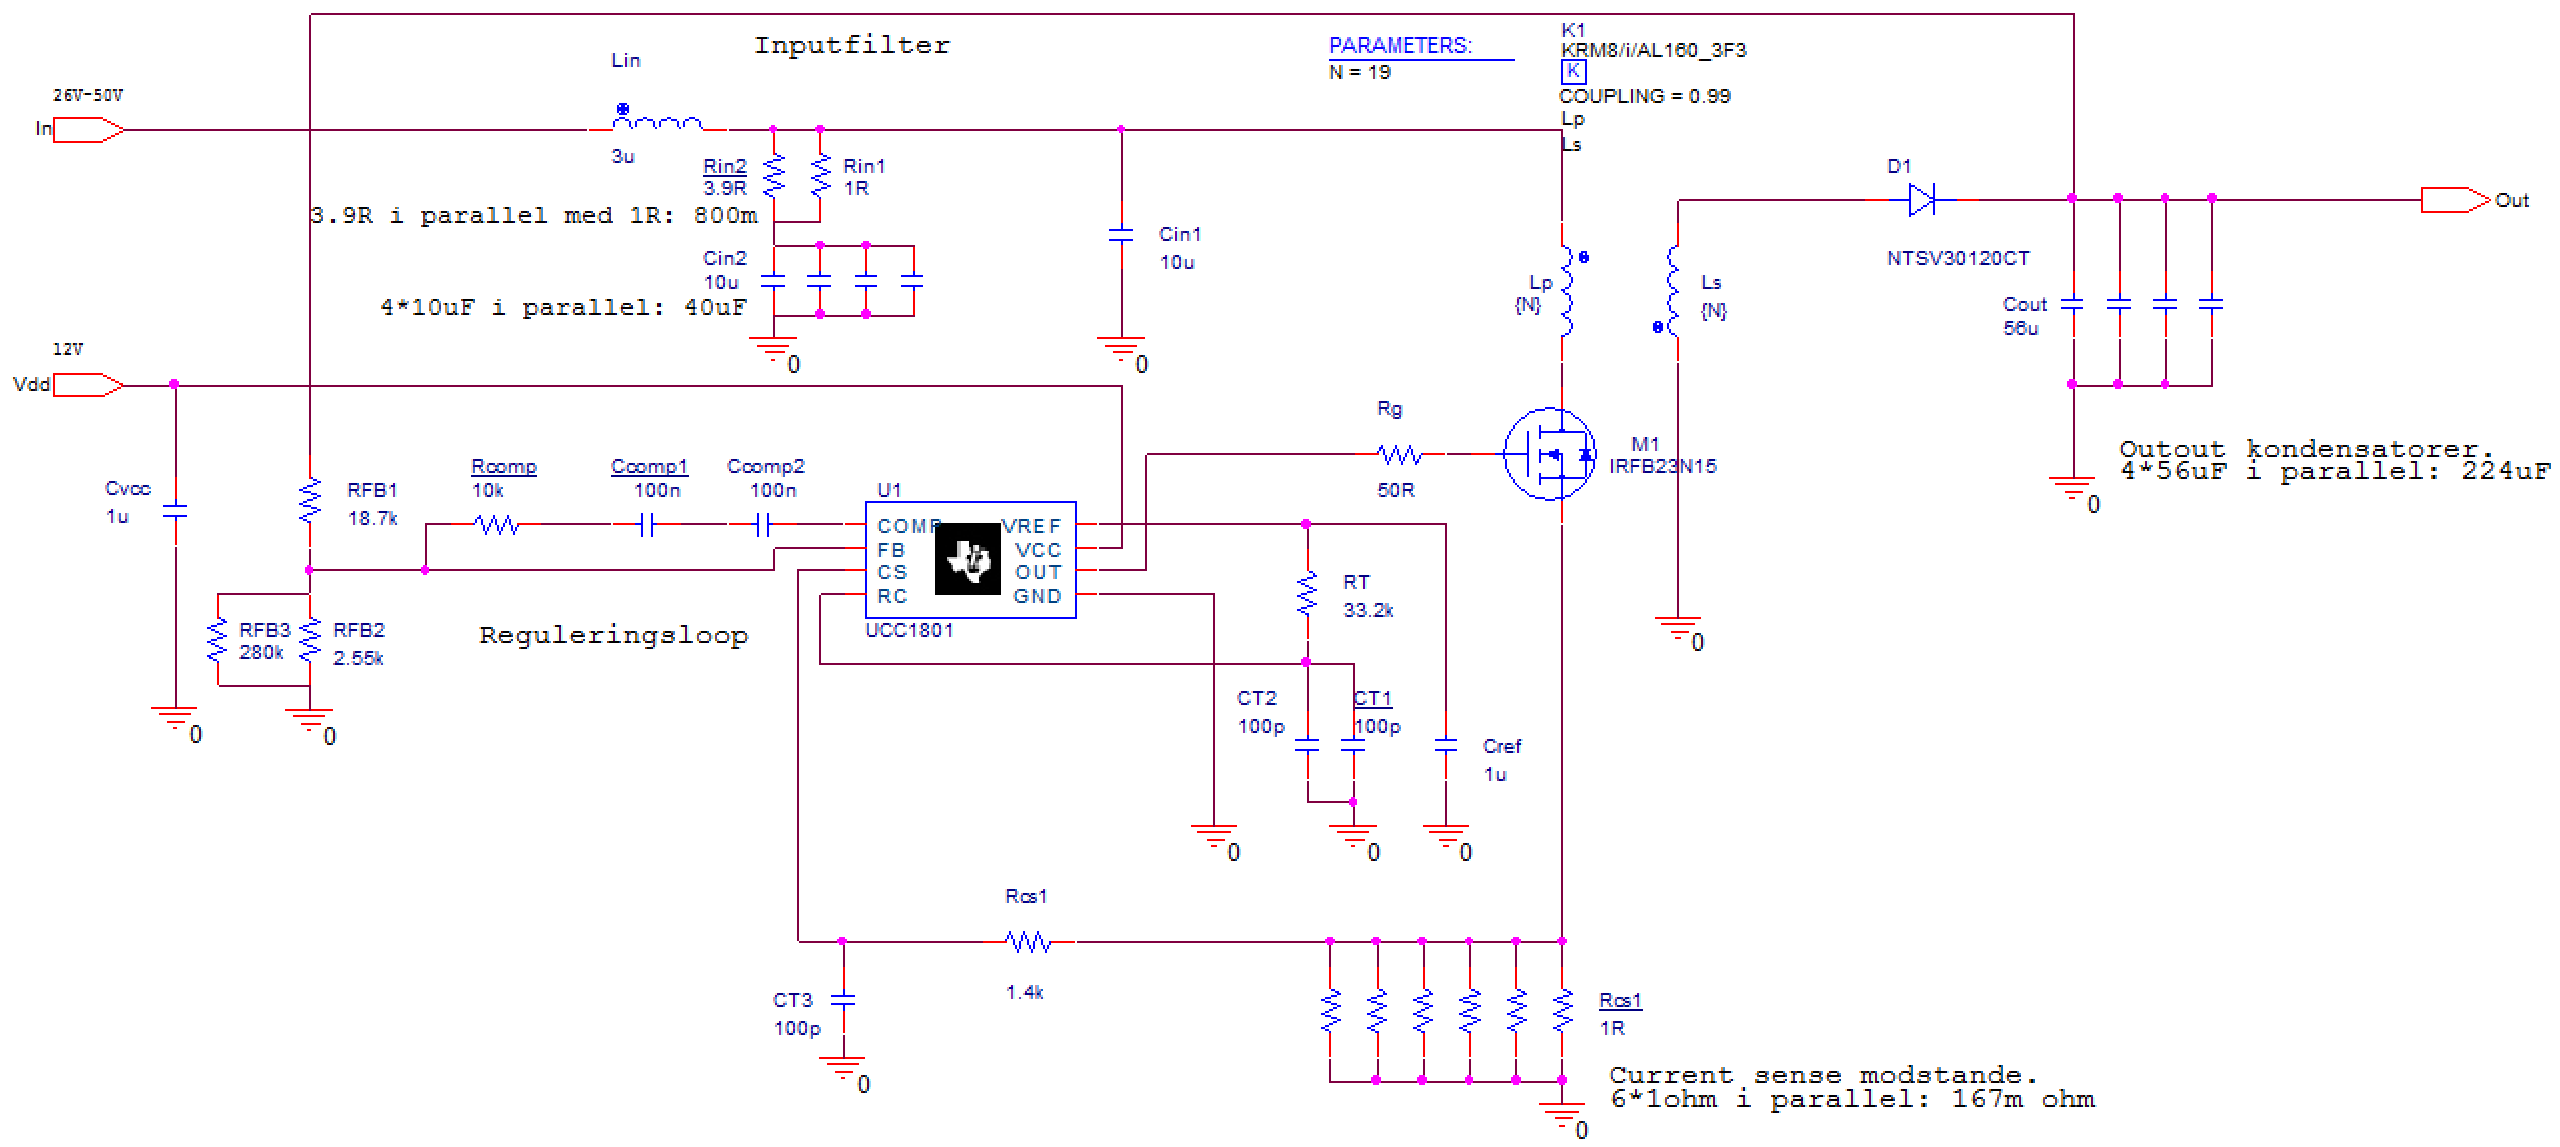
\includegraphics[max width=1.1\linewidth]{../dokumentation/tex/2iteration/billeder/Schemaricoverview_2iteration.PNG}
	\caption{Schematic overblik for 2. iteration}
	\label{fig:sche2iteration}
\end{figure}

\subsection{Constant-load}
Ved testen constant-load måles interessante steder i systemet, hvor en konstant belastning bruges. Her er en belastning på $8.4\ohm$ benyttet, med en indgangsspænding på 26V, med mindre andet er opgivet.

Ved testen er spændingen over outputtet, MOSFET'en og dioden målt. Desuden er der lavet målinger på de centrale dele af PWM-controlleren. Det indebærer målinger af switch-frekvensen, switch-tiden og stigetiden på filtret til current-sense signalet.  
Ved testen er converterens tab samtidig fundet. Tabet for transformator, MOSFET og diode er fået ved at måle temperaturen af den enkelte komponent, efter converteren har været kørende i længere tid. Temperaturstigningen er sammen med kølepladernes kølekoefficienter, og transformatorens termiske modstand, brugt til beregning af tab. Det samlede tab for converteren i 2. iteration, er i analyse og simulering fundet ved, at lægge de fundne tab sammen. I testen er der set på den effekt, der sendes ind i converteren og trukket udgangseffekten fra denne.

\subsection{Gain-fase måling}
Til gain-fase måling af converteren er Network Analyzeren HP4194A\cite{hp4194} benyttet. Her laves en måling af overføringsfunktionen for power-modul, fejlforstærker og for det samlede system. Det er gjort, ved at indføre et fejlsignal i tilbagekoblingen, og måle hvordan udgangen ændrer sig. Fejlsignalet blev indført med en amplitude på $30mV$. Dette er der lavet et frekvens-sweep på fra, $10\Hz$ til $100kHz$. Målingerne fra Network Analyzeren overføres til et Excel ark, hvor et bode plot er udarbejdet ud fra testmålingerne. 

\subsection{Load-step}
For at lave load-step testen, er der som udgangsbelastning brugt to $20\ohm$ modstande i parallel. Den ene koblet til en switch, så den kan kobles til eller fra. Det gør, at når switchen er OFF, består belastningen af en $20\ohm$ modstand. Når switchen er ON, består den i stedet af en $10\ohm$ modstand. Switchen var indstillet til at sende en puls på 10ms.

\noindent Ved denne test er det spændingsændringen på outputtet der er målt.